\documentclass[12pt,a4paper]{article}

% === Packages ===
\usepackage[utf8]{inputenc}
\usepackage[T1]{fontenc}
\usepackage{lmodern}
\usepackage[english]{babel}
\usepackage{amsmath,amssymb,amsthm}
\usepackage{graphicx}
\usepackage{booktabs}
\usepackage{hyperref}
\usepackage[margin=2.5cm]{geometry}
\usepackage{natbib}
\usepackage{algorithm}
\usepackage{algpseudocode}
\usepackage{listings}
\usepackage{xcolor}
\usepackage{float}
\usepackage{caption}
\usepackage{subcaption}
\usepackage{tikz}
\usetikzlibrary{arrows.meta,positioning,shapes.geometric,calc}

% === Hyperref config ===
\hypersetup{
    colorlinks=true,
    linkcolor=blue!60!black,
    citecolor=green!50!black,
    urlcolor=blue!70!black,
    pdftitle={Functional Pathway-Centric Medical Knowledge Graph with Exclusion Logic},
    pdfauthor={Lukas Geiger},
}

% === Listings config ===
\lstset{
    basicstyle=\ttfamily\small,
    backgroundcolor=\color{gray!8},
    frame=single,
    framerule=0.4pt,
    breaklines=true,
    captionpos=b,
}

% === Theorem environments ===
\newtheorem{definition}{Definition}
\newtheorem{theorem}{Theorem}
\newtheorem{proposition}{Proposition}

% === Title ===
\title{%
    \textbf{Functional Pathway-Centric Medical Knowledge Graph\\
    with Exclusion Logic}\\[0.5em]
    \large A System-Medicine Architecture for Differential Diagnosis Support
}
\author{
    Lukas Geiger\\
    Independent Researcher, Bernau, Germany\\
    ORCID: \url{https://orcid.org/0009-0005-7296-1534}
}
\date{March 2026 --- Concept Paper v0.2}

\begin{document}

\maketitle

% ================================================================
\begin{abstract}
We present the design and prototype implementation of a functional pathway-centric medical knowledge graph intended to support differential diagnosis. Standard clinical decision support systems organize knowledge around diagnoses, symptoms, or genes as primary entities. In contrast, the proposed system uses \emph{biological functional pathways} as its central organizing principle, linking genes, proteins, laboratory values, anatomical locations, cell types, and clinical diagnoses as secondary annotations.

This architecture enables a novel form of \emph{exclusion reasoning}: if a functional pathway is demonstrated to be intact (via normal laboratory markers), all genes essential and sufficient for that pathway can be excluded as primary causes of disease in the current patient. The system is implemented as a SQLite-backed prototype with a PySide6 graphical interface, integrating public data sources (Reactome, Gene Ontology, UniProt, HGNC, Uberon, Cell Ontology).

We describe the formal exclusion model---both binary and probabilistic variants---its assumptions and limitations, and propose a validation framework. The prototype is demonstrated on a hemolysis--immunodeficiency scenario involving five functional pathways, eleven genes, and seven laboratory markers. The system is positioned as a research tool for exploring the pathway-centric paradigm, not as a clinical decision support system.
\end{abstract}

\smallskip
\noindent\textbf{Keywords:} knowledge graph, differential diagnosis, functional pathways, exclusion reasoning, system medicine, Reactome, Gene Ontology

% ================================================================
\section{Introduction and Motivation}
\label{sec:introduction}

Differential diagnosis in complex, multi-system diseases frequently fails not from lack of data but from the inability to systematically integrate heterogeneous evidence. A patient with abnormal laboratory values may have hundreds of candidate genetic causes; current clinical tools largely present these as ranked lists without exploiting the logical structure of \emph{excluded} possibilities.

The central observation motivating this work is:

\begin{quote}
\emph{If a biological functional pathway is demonstrably intact, then all genes that are both necessary and sufficient for that pathway can be excluded as primary causes of dysfunction.}
\end{quote}

This transforms positive evidence (intact pathway) into negative diagnostic constraints (excluded genes), potentially reducing the candidate space substantially before differential diagnosis is applied.

Existing systems organize knowledge differently. PhenoTips \citep{Girdea2013} and Phenomizer \citep{Kohler2009} match patient phenotypes to disease databases via the Human Phenotype Ontology \citep{Robinson2008}. These systems excel at symptom-to-disease matching but do not exploit pathway integrity as exclusion evidence. Pathway databases such as Reactome \citep{Fabregat2018} and KEGG organize around biochemical reactions but are not designed for clinical exclusion reasoning. Gene Ontology \citep{Ashburner2000} provides fine-grained process descriptions but lacks the clinical decision framework.

The proposed system bridges this gap by treating functional pathways as \emph{first-class entities} in a knowledge graph, with all other biomedical concepts---genes, anatomical locations, cell types, laboratory markers, and diagnoses---attached as secondary annotations. This structural choice enables a formal exclusion logic that is both computationally tractable and biologically meaningful.

\subsection{Contributions}

\begin{enumerate}
    \item A \textbf{data model} centering on functional pathways as the primary organizing principle for clinical reasoning, linking six entity types through semantically typed edges.
    \item A \textbf{formal exclusion framework} with both binary and probabilistic variants, enabling systematic elimination of candidate genes based on pathway integrity evidence.
    \item A \textbf{prototype implementation} with data ingestion from six public biological databases, an interactive graph explorer, and a diagnosis query engine.
    \item A \textbf{validation framework} specifying metrics, benchmark requirements, and comparison criteria for evaluating the approach.
\end{enumerate}

% ================================================================
\section{Problem Statement and Formal Hypothesis}
\label{sec:problem}

\subsection{Formal Problem Statement}

Let $\mathcal{P} = \{p_1, \ldots, p_n\}$ be the set of biological functional pathways for a given patient context. Let $\mathcal{G}$ be the set of candidate genes. Let $\mathcal{E}(p_i) \subseteq \mathcal{G}$ be the set of genes \emph{essential} to pathway~$p_i$. Let $s(p_i) \in \{0, 1\}$ be the observed pathway status: $1 = \text{intact}$, $0 = \text{disrupted or unknown}$.

\begin{definition}[Binary Exclusion Rule]
\label{def:binary}
If $s(p_i) = 1$, then $\forall\, g \in \mathcal{E}(p_i)$: gene~$g$ is \emph{excluded} as a primary cause of disease, provided $g$ is essential only in pathways that are all intact:
\begin{equation}
    \text{excluded}(g) \iff \forall\, p_i \text{ s.t. } g \in \mathcal{E}(p_i): s(p_i) = 1
\end{equation}
\end{definition}

\begin{definition}[Probabilistic Exclusion Score]
\label{def:probabilistic}
For a gene~$g$, the exclusion confidence is:
\begin{equation}
    \text{excl}(g) = \prod_{i:\, g \in \mathcal{E}(p_i)} c(p_i) \cdot b(g)
\end{equation}
where $c(p_i) \in [0,1]$ is the pathway status confidence (intact: $0.95$, unknown: $0.50$, disrupted: $0.05$), and $b(g) \in [0,1]$ is a multi-pathway bonus factor:
\begin{equation}
    b(g) = \min\!\Big(1.0,\; 0.7 + 0.1 \cdot |\{p_i : g \in \mathcal{E}(p_i) \wedge s(p_i) = 1\}|\Big)
\end{equation}
The \emph{suspicion score} incorporates gene redundancy:
\begin{equation}
    \text{susp}(g) = \big(1 - \text{excl}(g)\big) \cdot r(g)
\end{equation}
where $r(g) \in \{1.0, 0.85, 0.6, 0.3\}$ maps the gene's redundancy degree (none, low, medium, high).
\end{definition}

\subsection{Core Hypothesis}

\begin{quote}
\emph{Pathway-status-based exclusion logic systematically reduces the candidate gene set for complex rare disease cases by at least 30\% relative to phenotype-only filtering, when evaluated on a curated benchmark dataset.}
\end{quote}

This is a specific, falsifiable hypothesis. The 30\% threshold is set as a minimal clinically meaningful reduction; a null result ($<10\%$ reduction) would indicate that the exclusion logic adds little diagnostic value beyond existing tools.

The candidate reduction rate (CRR) is defined as:
\begin{equation}
    \text{CRR} = 1 - \frac{|\mathcal{G}_{\text{after exclusion}}|}{|\mathcal{G}_{\text{before exclusion}}|}
\end{equation}

% ================================================================
\section{System Architecture}
\label{sec:architecture}

\subsection{Data Model}
\label{sec:datamodel}

The central entity is the \textbf{FunctionalPathway} node, representing a discrete biological process with observable inputs and outputs. Figure~\ref{fig:schema} illustrates the complete data model.

\begin{figure}[H]
\centering
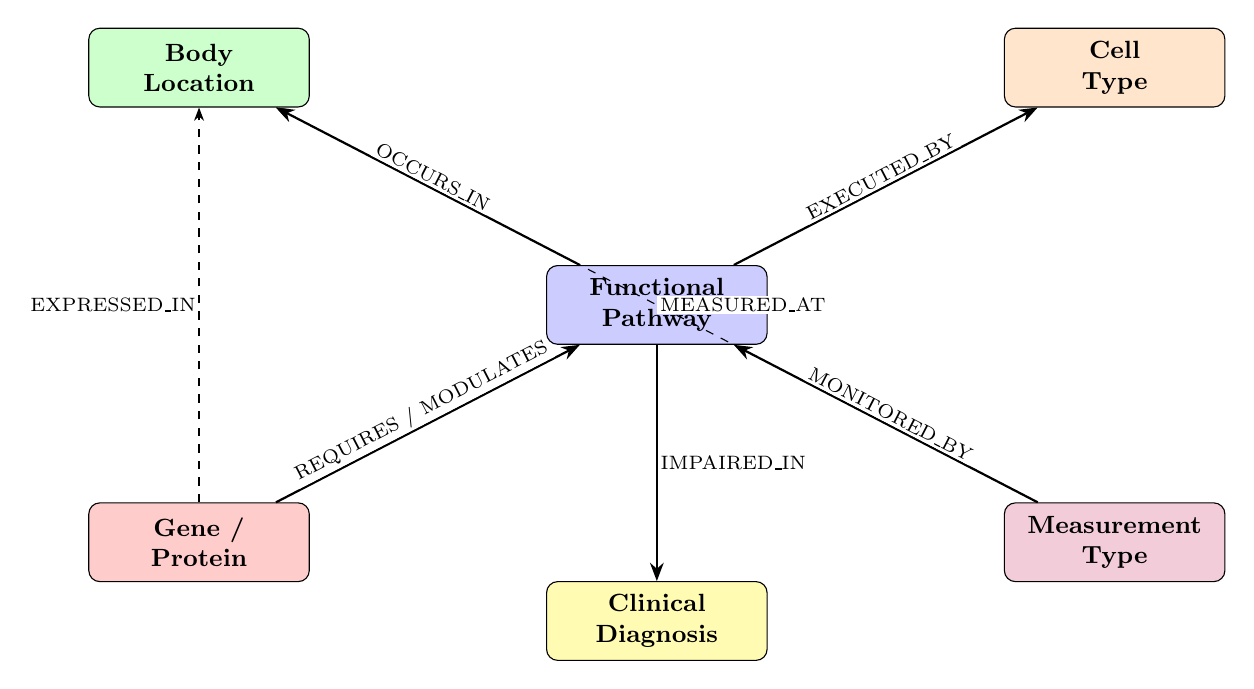
\begin{tikzpicture}[
    entity/.style={draw, rounded corners, minimum width=2.8cm, minimum height=1cm, font=\small\bfseries, align=center},
    edge_label/.style={font=\scriptsize, fill=white, inner sep=1pt},
    >=Stealth,
    node distance=2.5cm and 3cm
]
    % Central node
    \node[entity, fill=blue!20] (pathway) {Functional\\Pathway};

    % Surrounding nodes
    \node[entity, fill=green!20, above left=2cm and 3cm of pathway] (location) {Body\\Location};
    \node[entity, fill=orange!20, above right=2cm and 3cm of pathway] (cell) {Cell\\Type};
    \node[entity, fill=red!20, below left=2cm and 3cm of pathway] (gene) {Gene /\\Protein};
    \node[entity, fill=purple!20, below right=2cm and 3cm of pathway] (measurement) {Measurement\\Type};
    \node[entity, fill=yellow!30, below=3cm of pathway] (diagnosis) {Clinical\\Diagnosis};

    % Edges
    \draw[->, thick] (pathway) -- node[edge_label, above, sloped] {OCCURS\_IN} (location);
    \draw[->, thick] (pathway) -- node[edge_label, above, sloped] {EXECUTED\_BY} (cell);
    \draw[->, thick] (gene) -- node[edge_label, above, sloped] {REQUIRES / MODULATES} (pathway);
    \draw[->, thick] (measurement) -- node[edge_label, above, sloped] {MONITORED\_BY} (pathway);
    \draw[->, thick] (pathway) -- node[edge_label, right] {IMPAIRED\_IN} (diagnosis);

    % Cross-edges
    \draw[->, dashed] (gene) -- node[edge_label, left] {EXPRESSED\_IN} (location);
    \draw[->, dashed] (measurement) -- node[edge_label, right] {MEASURED\_AT} (location);
\end{tikzpicture}
\caption{Entity-relationship diagram of the pathway-centric knowledge graph. Solid arrows indicate primary relationships through the pathway hub; dashed arrows indicate secondary cross-links.}
\label{fig:schema}
\end{figure}

Each entity type carries domain-specific attributes:

\begin{itemize}
    \item \textbf{FunctionalPathway}: name, description, primary output, temporal class (acute/chronic), status (intact/disrupted/unknown), external~ID (Reactome or GO).
    \item \textbf{BodyLocation} (Uberon): organ, subcompartment, circulation type, immune role.
    \item \textbf{CellType} (Cell Ontology): lineage, maturation stage, lifespan, mobility.
    \item \textbf{Gene/Protein} (HGNC/UniProt): symbol, function type (structural, regulatory, signaling, metabolic), redundancy degree, expression sites.
    \item \textbf{MeasurementType}: name, LOINC code, reference range, measurement site, sensitivity, specificity.
    \item \textbf{ClinicalDiagnosis}: name, ICD-10 code, description.
\end{itemize}

Edge types carry semantic labels (Table~\ref{tab:edges}) and, for gene--pathway edges, an \texttt{is\_essential} flag that distinguishes modulatory from essential gene contributions.

\begin{table}[H]
\centering
\caption{Semantic edge types in the knowledge graph.}
\label{tab:edges}
\begin{tabular}{lll}
\toprule
\textbf{Source} & \textbf{Target} & \textbf{Relation} \\
\midrule
Pathway & BodyLocation & \texttt{OCCURS\_IN} \\
Pathway & CellType & \texttt{EXECUTED\_BY} \\
Gene & Pathway & \texttt{REQUIRES} (essential) / \texttt{MODULATES} \\
Measurement & Pathway & \texttt{MONITORS\_OUTPUT\_OF} \\
Measurement & BodyLocation & \texttt{REPRESENTS\_ACTIVITY\_IN} \\
Pathway & Diagnosis & \texttt{DISRUPTION\_LEADS\_TO} \\
Gene & BodyLocation & \texttt{EXPRESSED\_IN} \\
\bottomrule
\end{tabular}
\end{table}

\subsection{Implementation}
\label{sec:implementation}

The prototype uses \textbf{SQLite} as the backend, with relational tables simulating a graph structure through association tables (Figure~\ref{fig:schema_sql}). The system comprises four main modules:

\begin{enumerate}
    \item \textbf{Ingestion module}: Downloads and parses six public data sources (Section~\ref{sec:datasources}), with a manifest-based tracking system to avoid redundant downloads.
    \item \textbf{Engine module}: Implements the exclusion logic (binary and probabilistic), graph traversal queries, pattern detection for measurement signatures, and human-readable explanation generation.
    \item \textbf{GUI module}: A PySide6-based desktop application with four tabs: Graph Explorer (interactive network visualization via NetworkX), Exclusion Panel (pathway status management and analysis), Diagnosis Query (measurement-driven hypothesis generation), and Data Browser (raw table inspection).
    \item \textbf{Database module}: Schema definition, CRUD helpers, and edge-linking functions with foreign key constraints.
\end{enumerate}

\begin{figure}[H]
\centering
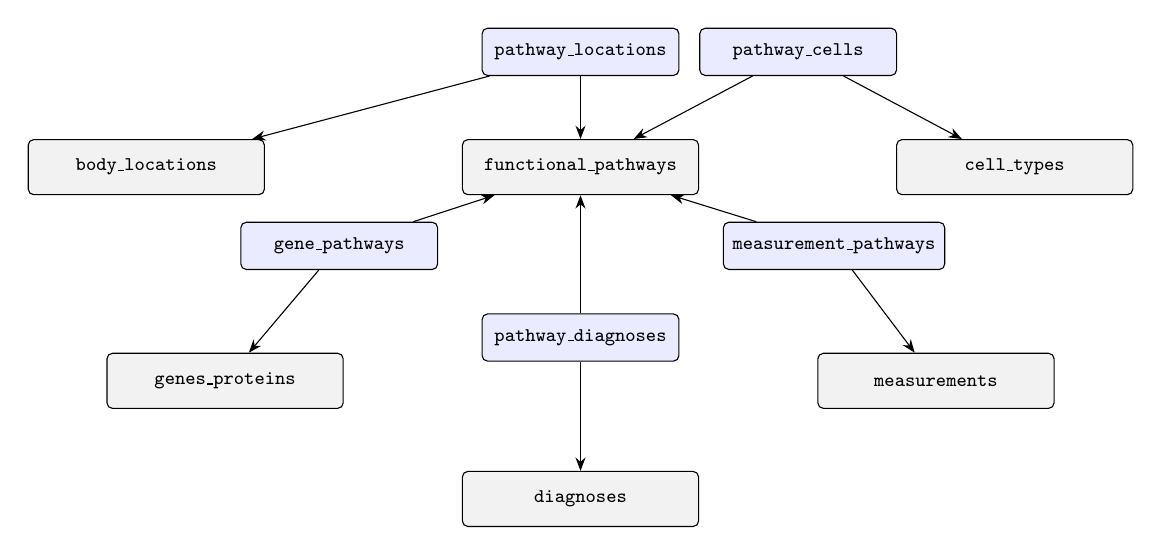
\begin{tikzpicture}[
    table/.style={draw, rounded corners=2pt, minimum width=3cm, minimum height=0.7cm, font=\ttfamily\scriptsize, fill=gray!10},
    assoc/.style={draw, rounded corners=2pt, minimum width=2.5cm, minimum height=0.6cm, font=\ttfamily\scriptsize, fill=blue!8},
    >=Stealth,
    node distance=1.2cm
]
    \node[table] (fp) {functional\_pathways};
    \node[table, left=2.5cm of fp] (bl) {body\_locations};
    \node[table, right=2.5cm of fp] (ct) {cell\_types};
    \node[table, below left=2cm and 1.5cm of fp] (gp) {genes\_proteins};
    \node[table, below right=2cm and 1.5cm of fp] (ms) {measurements};
    \node[table, below=3.5cm of fp] (dg) {diagnoses};

    \node[assoc, above=0.8cm of fp] (pl) {pathway\_locations};
    \node[assoc, above right=0.8cm and 0cm of fp] (pc) {pathway\_cells};
    \node[assoc, left=0.3cm of fp, yshift=-1cm] (gpw) {gene\_pathways};
    \node[assoc, right=0.3cm of fp, yshift=-1cm] (mp) {measurement\_pathways};
    \node[assoc, below=1.5cm of fp] (pd) {pathway\_diagnoses};

    \draw[->] (pl) -- (fp);
    \draw[->] (pl) -- (bl);
    \draw[->] (pc) -- (fp);
    \draw[->] (pc) -- (ct);
    \draw[->] (gpw) -- (gp);
    \draw[->] (gpw) -- (fp);
    \draw[->] (mp) -- (ms);
    \draw[->] (mp) -- (fp);
    \draw[->] (pd) -- (fp);
    \draw[->] (pd) -- (dg);
\end{tikzpicture}
\caption{SQLite relational schema. Gray boxes are entity tables; blue boxes are association (edge) tables with foreign keys.}
\label{fig:schema_sql}
\end{figure}

A dedicated \textbf{Graph Explorer} (NetworkX-based) visualizes subgraphs with lazy-loaded neighborhoods. Graph layout is computed in a background thread to maintain GUI responsiveness. Nodes are color-coded by entity type; pathway nodes additionally display their status (intact/disrupted/unknown) through border colors.

\paragraph{Note on graph database choice.} The current SQLite implementation enables rapid prototyping but introduces known limitations for deep graph traversal (see Section~\ref{sec:limitations}). A production system would benefit from Neo4j or a comparable native graph database. The prototype demonstrates the conceptual model; performance comparisons with graph-native backends are planned.

\subsection{Data Sources}
\label{sec:datasources}

The system integrates six public biological databases, each contributing a specific entity type to the knowledge graph:

\begin{table}[H]
\centering
\caption{Integrated data sources and their roles.}
\label{tab:datasources}
\begin{tabular}{llll}
\toprule
\textbf{Source} & \textbf{Entity Type} & \textbf{Format} & \textbf{Status} \\
\midrule
Reactome \citep{Fabregat2018} & Pathways, reactions & TSV & Integrated \\
Gene Ontology \citep{Ashburner2000} & Biological processes & OBO, GAF & Integrated \\
UniProt \citep{UniProt2023} & Proteins, gene links & TSV & Integrated \\
HGNC \citep{Braschi2019} & Gene nomenclature & TSV & Integrated \\
Uberon \citep{Mungall2012} & Anatomical locations & OBO & Integrated \\
Cell Ontology \citep{Diehl2016} & Cell types & OBO & Integrated \\
OMIM / HPO \citep{Robinson2008} & Disease--gene links & --- & Planned \\
\bottomrule
\end{tabular}
\end{table}

Data ingestion follows a defined order (HGNC $\to$ Uberon $\to$ Cell Ontology $\to$ UniProt $\to$ Reactome $\to$ GO) to satisfy foreign key dependencies. Each source is tracked via a manifest file recording download timestamps, SHA-256 checksums, and import status.

% ================================================================
\section{Exclusion Logic}
\label{sec:exclusion}

\subsection{Binary Exclusion}

The binary exclusion engine (Definition~\ref{def:binary}) iterates over all genes marked as essential in at least one pathway. For each gene, it retrieves all pathways where the gene is essential and checks whether \emph{all} of these pathways have status ``intact.'' If so, the gene is excluded; otherwise, it remains a candidate.

\begin{algorithm}[H]
\caption{Binary Exclusion Analysis}
\label{alg:binary}
\begin{algorithmic}[1]
\Require Set of pathways $\mathcal{P}$ with status $s(p_i)$, essential gene mapping $\mathcal{E}$
\Ensure Sets $\mathcal{G}_{\text{excluded}}$, $\mathcal{G}_{\text{candidate}}$
\State $\mathcal{I} \gets \{p_i \in \mathcal{P} : s(p_i) = \text{intact}\}$
\ForAll{$g \in \bigcup_{p \in \mathcal{P}} \mathcal{E}(p)$} \Comment{All essential genes}
    \State $P_g \gets \{p \in \mathcal{P} : g \in \mathcal{E}(p)\}$ \Comment{Pathways requiring $g$}
    \If{$P_g \subseteq \mathcal{I}$ \textbf{and} $P_g \neq \emptyset$}
        \State $\mathcal{G}_{\text{excluded}} \gets \mathcal{G}_{\text{excluded}} \cup \{g\}$
    \Else
        \State $\mathcal{G}_{\text{candidate}} \gets \mathcal{G}_{\text{candidate}} \cup \{g\}$
    \EndIf
\EndFor
\end{algorithmic}
\end{algorithm}

The confidence of exclusion depends on the number of intact pathways: a gene excluded via multiple independent intact pathways has stronger evidence than one excluded via a single pathway.

\subsection{Probabilistic Exclusion}

The probabilistic engine (Definition~\ref{def:probabilistic}) extends the binary model by assigning continuous confidence scores. Three factors contribute:

\begin{enumerate}
    \item \textbf{Pathway evidence}: Each pathway status maps to a confidence value (intact: $0.95$, unknown: $0.50$, disrupted: $0.05$). The combined pathway confidence for a gene is the product over all its essential pathways.
    \item \textbf{Multi-pathway bonus}: Genes essential in multiple intact pathways receive a bonus factor, reflecting stronger evidence from independent sources.
    \item \textbf{Redundancy weighting}: The suspicion score is modulated by the gene's redundancy degree. Genes with no functional backup (redundancy = ``none'') receive full suspicion weight ($r = 1.0$); highly redundant genes receive reduced weight ($r = 0.3$).
\end{enumerate}

Genes are categorized by exclusion confidence: high ($\geq 0.8$), moderate ($0.3$--$0.8$), or suspect ($< 0.3$). This tripartite classification provides clinicians with a ranked prioritization rather than a binary decision.

\subsection{Pattern Detection}

In addition to exclusion reasoning, the system implements \textbf{measurement signature detection}. A signature is a predefined pattern of abnormal laboratory values (e.g., ``hemolysis signature'': low haptoglobin + high LDH + high indirect bilirubin + high reticulocytes + low hemoglobin). Each component carries a weight reflecting its diagnostic importance.

Given a set of abnormal measurements, the system computes a weighted match score against all defined signatures:
\begin{equation}
    \text{match}(S) = \frac{\sum_{c \in S_{\text{matched}}} w_c}{\sum_{c \in S_{\text{all}}} w_c}
\end{equation}
Signatures with $\text{match} \geq 0.3$ are reported, enabling rapid identification of known clinical patterns.

% ================================================================
\section{Demonstration: Hemolysis--Immunodeficiency Scenario}
\label{sec:demo}

The prototype includes a curated seed dataset modeling the intersection of hereditary spherocytosis, autoimmune hemolytic anemia, and agammaglobulinemia. This scenario was chosen because it involves multiple interacting pathways with shared anatomical locations (spleen, bone marrow) and demonstrates the exclusion logic across independent functional domains.

\subsection{Functional Pathways}

Five pathways are modeled (Table~\ref{tab:pathways}), spanning two clinical domains (hematology and immunology) with distinct temporal characteristics.

\begin{table}[H]
\centering
\caption{Functional pathways in the demonstration scenario.}
\label{tab:pathways}
\begin{tabular}{lll}
\toprule
\textbf{Pathway} & \textbf{Output} & \textbf{Temporal} \\
\midrule
Erythrocyte membrane integrity & Stable biconcave RBCs & Chronic \\
Erythrocyte degradation (hemolysis) & Free Hb $\to$ bilirubin & Acute \\
Splenic filtration & Removal of defective cells & Acute \\
Early B-cell differentiation & Functional pre-B cells & Chronic \\
Antibody production & IgG, IgM, IgA & Both \\
\bottomrule
\end{tabular}
\end{table}

\subsection{Gene--Pathway Essentiality}

Eleven genes are linked to these pathways with explicit essentiality annotations (Table~\ref{tab:genes}). The essentiality flag is the critical attribute enabling exclusion logic: only essential genes can be excluded when their pathway is intact.

\begin{table}[H]
\centering
\caption{Genes and their pathway essentiality in the demonstration scenario.}
\label{tab:genes}
\begin{tabular}{llll}
\toprule
\textbf{Gene} & \textbf{Pathway} & \textbf{Essential} & \textbf{Redundancy} \\
\midrule
ANK1 & Membrane integrity & Yes & None \\
SLC4A1 & Membrane integrity & Yes & None \\
SPTA1 & Membrane integrity & Yes & Low \\
SPTB & Membrane integrity & Yes & None \\
EPB42 & Membrane integrity & Yes & Low \\
HMOX1 & Hemolysis & Yes & Low \\
HP & Hemolysis & No & Low \\
BLNK & B-cell differentiation & Yes & None \\
CD19 & B-cell differentiation & Yes & None \\
PAX5 & B-cell differentiation & Yes & None \\
NOTCH2 & Splenic filtration, B-cell diff. & Yes / No & Low \\
\bottomrule
\end{tabular}
\end{table}

\subsection{Exclusion Scenario}

Consider a patient presenting with:
\begin{itemize}
    \item Low hemoglobin (anemia)
    \item Low haptoglobin (hemolysis marker)
    \item High LDH, high indirect bilirubin (hemolysis)
    \item Normal B-cell count (CD19+)
    \item Normal IgG levels
\end{itemize}

The system derives:
\begin{enumerate}
    \item Normal B-cell count $\Rightarrow$ B-cell differentiation pathway \emph{intact} $\Rightarrow$ \textbf{exclude} BLNK, CD19, PAX5.
    \item Normal IgG $\Rightarrow$ antibody production pathway \emph{intact}.
    \item Hemolysis markers abnormal $\Rightarrow$ hemolysis pathway \emph{disrupted}.
    \item NOTCH2 is essential in splenic filtration (status unknown) and non-essential in B-cell differentiation $\Rightarrow$ \textbf{remains candidate}.
    \item Membrane genes (ANK1, SLC4A1, SPTA1, SPTB, EPB42) are essential only in the membrane integrity pathway (status unknown/disrupted) $\Rightarrow$ \textbf{remain candidates}.
\end{enumerate}

Result: 3 of 10 essential genes excluded (CRR = 30\%), matching the hypothesis threshold. The remaining candidates correctly include the membrane-structural genes associated with hereditary spherocytosis.

% ================================================================
\section{Assumptions and Limitations}
\label{sec:limitations}

\subsection{Independence Assumption}

The binary exclusion model assumes that pathways are \emph{functionally independent}: an intact pathway~$p_i$ excludes its essential genes regardless of the status of other pathways. This assumption is \textbf{known to be false} in many biological contexts:

\begin{itemize}
    \item Many genes participate in multiple pathways (\emph{pleiotropy}). A gene excluded via pathway~$p_i$ may still be causative via a different pathway~$p_j$ that is not assessed. The model addresses this by requiring \emph{all} pathways of a gene to be intact before exclusion.
    \item Compensatory mechanisms can maintain measured pathway outputs even when an essential gene is partially dysfunctional.
    \item The binary status $s(p_i) \in \{0, 1\}$ is a simplification; real pathway activity exists on a continuum.
\end{itemize}

The probabilistic model partially mitigates these limitations through continuous confidence scores, but the weight parameters are currently assigned heuristically.

\subsection{Essentiality Definition}

``Essential gene'' is defined operationally as a gene annotated in Reactome or curated sources as \emph{required} for at least one reaction in the pathway. This definition is conservative and should be refined using curated essentiality databases (e.g., DepMap, CRISPR essentiality screens).

\subsection{Database Backend}

The SQLite implementation suffices for the current prototype ($\sim$17\,MB database, $<$2000 pathways) but introduces limitations for full-scale deployment:

\begin{itemize}
    \item Deep graph traversals (depth $>3$) require multiple JOIN operations that scale poorly.
    \item No native support for shortest-path or pattern-matching queries available in graph databases (e.g., Neo4j Cypher).
    \item Concurrent write access is limited by SQLite's file-level locking.
\end{itemize}

\subsection{Data Completeness}

Not all pathways have adequate Reactome coverage. Orphan pathways, tissue-specific metabolism, and recently characterized mechanisms may not be represented. The Gene Ontology integration adds breadth but at the cost of granularity---many GO biological process terms are too generic to serve as meaningful functional pathways.

\subsection{EHR Interoperability}

A practical deployment of exclusion-based clinical decision support requires integration with electronic health record (EHR) systems to obtain structured patient laboratory data. Without interoperable access to real-time laboratory values via standards such as HL7 FHIR, the system remains limited to manually entered measurements. EHR interoperability is a well-documented challenge in clinical informatics; addressing it is beyond the scope of this concept paper but constitutes a critical requirement for any future clinical application.

\subsection{Measurement Redundancy and Contextuality}

The probabilistic exclusion formula (Definition~\ref{def:probabilistic}) assumes that laboratory measurements provide independent evidence about pathway status. However, Dzhafarov and Kujala's Contextuality-by-Default (CbD) framework \citep{Dzhafarov2016} warns that parallel measurements may exhibit informational redundancy rather than genuine independence. When two laboratory values decline simultaneously, this may reflect redundant measurement of the same pathway output rather than independent evidence of a shared genetic cause (pleiotropy). A rigorous treatment would require a CbD-inspired correction term in the exclusion score that accounts for measurement context overlap. This refinement is planned for future versions of the probabilistic model.

% ================================================================
\section{Related Work}
\label{sec:related}

\subsection{Phenotype-Driven Diagnosis Support}

Phenomizer \citep{Kohler2009} and PhenoTips \citep{Girdea2013} represent the state of the art in phenotype-driven diagnosis. Both systems match patient phenotypes (HPO terms) to disease databases and rank candidate diagnoses by semantic similarity. They are effective for symptom-to-disease matching but do not model biological pathways or exploit pathway integrity for exclusion reasoning.

\subsection{Pathway Analysis in Genomics}

Gene Set Enrichment Analysis (GSEA) \citep{Subramanian2005} and related tools identify dysregulated pathways from expression data. These methods operate at the population level and require omics data not typically available in routine clinical settings. The proposed system works with individual patient laboratory values, making it applicable in standard clinical workflows.

\subsection{Graph-Based Clinical Reasoning}

Knowledge graphs for clinical decision support have been explored in several contexts. Clinical knowledge graphs built from electronic health records \citep{Rotmensch2017} capture statistical associations between diagnoses, laboratory values, and treatments. Large-scale biomedical knowledge graphs such as Hetionet \citep{Himmelstein2017} integrate diverse data sources for drug repurposing and hypothesis generation. However, none of these systems use pathway status as a first-class constraint in exclusion reasoning.

\subsection{LLM-Augmented Biomedical Reasoning}

Recent work combines large language models with biomedical knowledge graphs. ESCARGOT \citep{Matsumoto2025} integrates LLMs with a dynamic ``Graph of Thoughts'' architecture and biomedical knowledge graphs for multihop reasoning tasks. While ESCARGOT demonstrates effective graph-based reasoning in biomedical contexts, it operates as a general-purpose reasoning agent without explicit exclusion logic. The proposed system shares the emphasis on knowledge graph-guided reasoning but differs fundamentally in its organizing principle: functional pathways as first-class diagnostic constraints rather than general-purpose graph traversal.

HealthGenie \citep{Gao2025} demonstrates knowledge-driven LLM integration for personalized health guidance. Its approach organizes knowledge graphs around user profiles and dietary recommendations---a symptom-centric (or need-centric) organization. In contrast, the proposed system organizes around biological functional pathways, enabling mechanistic exclusion reasoning that is not available in symptom-centric architectures.

\subsection{Comparison Summary}

\begin{table}[H]
\centering
\caption{Comparison of the proposed system with related approaches.}
\label{tab:comparison}
\begin{tabular}{lcccc}
\toprule
\textbf{System} & \textbf{Primary Entity} & \textbf{Exclusion} & \textbf{Lab Values} & \textbf{Pathways} \\
\midrule
Phenomizer & HPO phenotypes & No & No & No \\
PhenoTips & Patient phenotypes & No & Limited & No \\
GSEA/KEGG & Pathways & No & Omics only & Yes \\
Hetionet & Heterogeneous & No & No & Partial \\
Clinical KGs & EHR data & No & Yes & No \\
ESCARGOT & KG + LLM & No & No & Partial \\
HealthGenie & KG + LLM & No & No & No \\
\textbf{Proposed} & \textbf{Pathways} & \textbf{Yes} & \textbf{Yes} & \textbf{Yes} \\
\bottomrule
\end{tabular}
\end{table}

% ================================================================
\section{Evaluation Framework}
\label{sec:evaluation}

\subsection{Benchmark Dataset}

A rigorous validation requires a curated benchmark of 20--50 confirmed genetic diagnoses where:
\begin{enumerate}
    \item Patient laboratory profiles are available at the time of initial presentation (before genetic diagnosis).
    \item The genetic diagnosis is confirmed (variant + phenotype + functional study).
    \item The patient's pathway status can be retrospectively reconstructed from laboratory data.
\end{enumerate}

Target sources include rare disease registries (EURORDIS), OMIM clinical synopsis entries, and published case series with comprehensive laboratory workups.

\subsection{Primary Metric}

The candidate reduction rate (CRR, Equation~5) serves as the primary success criterion. A CRR $> 0.30$ supports the core hypothesis; a CRR $< 0.10$ would indicate insufficient diagnostic value.

\textbf{Safety constraint}: The confirmed causal gene must \emph{never} be excluded (false exclusion rate = 0). Any false exclusion in the benchmark invalidates the model for clinical application.

\subsection{Alternative Validation: Synthetic Patient Personas}

An alternative validation pathway addresses the scarcity of annotated real-world datasets for rare diseases. LLM-generated synthetic patient personas can be constructed by introducing targeted perturbations in the pathway graph---for example, simulating an ANK1 defect by setting the erythrocyte membrane integrity pathway to ``disrupted'' and deriving consistent laboratory values. Since the causal gene is defined \emph{a priori}, the exclusion engine can be evaluated with exact ground truth: the system must exclude non-causal genes (measuring CRR) while never excluding the planted causal gene (measuring false exclusion rate). This approach complements the real-case benchmark and permits systematic testing across a wider range of disease scenarios than may be available from registries alone.

\subsection{Secondary Metrics}

\begin{itemize}
    \item \textbf{Rank improvement}: Position of the correct gene in the ranked candidate list after exclusion filtering.
    \item \textbf{Coverage}: Percentage of benchmark cases where at least one pathway can be assessed from available laboratory data.
    \item \textbf{Comparison}: CRR versus standard HPO-only filtering on the same case set.
\end{itemize}

% ================================================================
\section{Discussion}
\label{sec:discussion}

The pathway-centric approach addresses a structural gap in current clinical decision support: the systematic use of \emph{negative evidence} (what is demonstrably working) to constrain the diagnostic space. This is conceptually analogous to industrial fault diagnosis, where functioning subsystems eliminate entire branches of the fault tree.

Several design decisions merit discussion:

\paragraph{Why pathways as center, not genes or diagnoses?} Genes are causes; diagnoses are consequences. Neither provides the mechanistic intermediate layer needed for exclusion reasoning. Pathways represent the functional units that connect genetic causes to clinical effects, making them the natural pivot for both inclusion and exclusion logic.

\paragraph{Binary vs.\ probabilistic exclusion.} The binary model is conceptually simpler and easier to validate (a gene is either excluded or not), but it cannot express uncertainty. The probabilistic model captures graded evidence but requires calibrated parameters. We recommend the binary model for initial validation and the probabilistic model for clinical exploration.

\paragraph{Scalability.} The current prototype handles the demonstration scenario ($\sim$50 nodes, $\sim$80 edges) without performance concerns. Scaling to the full Reactome database ($>$2400 pathways, $>$10{,}000 reactions) will require performance testing and likely a migration to a graph database backend.

% ================================================================
\section{Conclusion and Future Work}
\label{sec:conclusion}

The functional pathway-centric knowledge graph represents a structurally distinct approach to differential diagnosis support, exploiting pathway-status evidence as explicit diagnostic constraints. The prototype implementation demonstrates feasibility across all core components: data ingestion from six public databases, graph modeling with semantic edge types, binary and probabilistic exclusion reasoning, pattern detection, and interactive visualization.

The core hypothesis---that pathway exclusion reduces the candidate gene space by $\geq 30\%$ without false exclusions---is testable and constitutes the primary empirical target for future work.

\subsection{Key Open Tasks}

\begin{enumerate}
    \item \textbf{Benchmark dataset}: Curate 20--50 cases from rare disease registries with laboratory profiles and confirmed genetic diagnoses.
    \item \textbf{Weight calibration}: Develop a data-driven method for estimating pathway confidence weights $c(p_i)$ from measurement reliability and pathway redundancy.
    \item \textbf{OMIM/HPO integration}: Link disease--gene associations from OMIM and HPO annotations to enable direct comparison with phenotype-only filtering.
    \item \textbf{Graph database migration}: Evaluate Neo4j or similar backends for scalability beyond the SQLite prototype.
    \item \textbf{Clinical tool comparison}: Benchmark against Phenomizer on the same case set to quantify the added value of pathway-centric exclusion.
    \item \textbf{Temporal modeling}: Extend the framework to capture disease progression and time-dependent pathway status changes.
\end{enumerate}

% ================================================================
\section*{Data and Software Availability}

The prototype source code, including database schema, ingestion pipelines, exclusion engines, and GUI application, is available as open-source software. The system integrates exclusively public data sources; no patient data is used or required.

% ================================================================
\section*{AI Disclosure}

AI-assisted tools (Claude, Anthropic) were used in the preparation of this manuscript, particularly for literature research, code development support, text structuring, and translation assistance. The conceptual design, scientific argumentation, formal model development, and responsibility for all content lie exclusively with the author.

% ================================================================
\bibliographystyle{apalike}
\bibliography{references}

\end{document}
